\section{Differential Datalog (DDlog)}\label{sec-ddlog}

\subsection{Differential computation}

A DDlog program operates on typed collections, or relations.  The
programmer defines a set of rules to compute a set of output relations
based on input relations (Figure~\ref{fig:differential}).  Rules are
evaluated incrementally: given a set of \emph{changes} to the input
collections (insertions or deletions), DDlog produces a set of changes
to the output collections (expressed also as insertions or deletions).

\begin{figure}
  \begin{minipage}{.48\textwidth}
    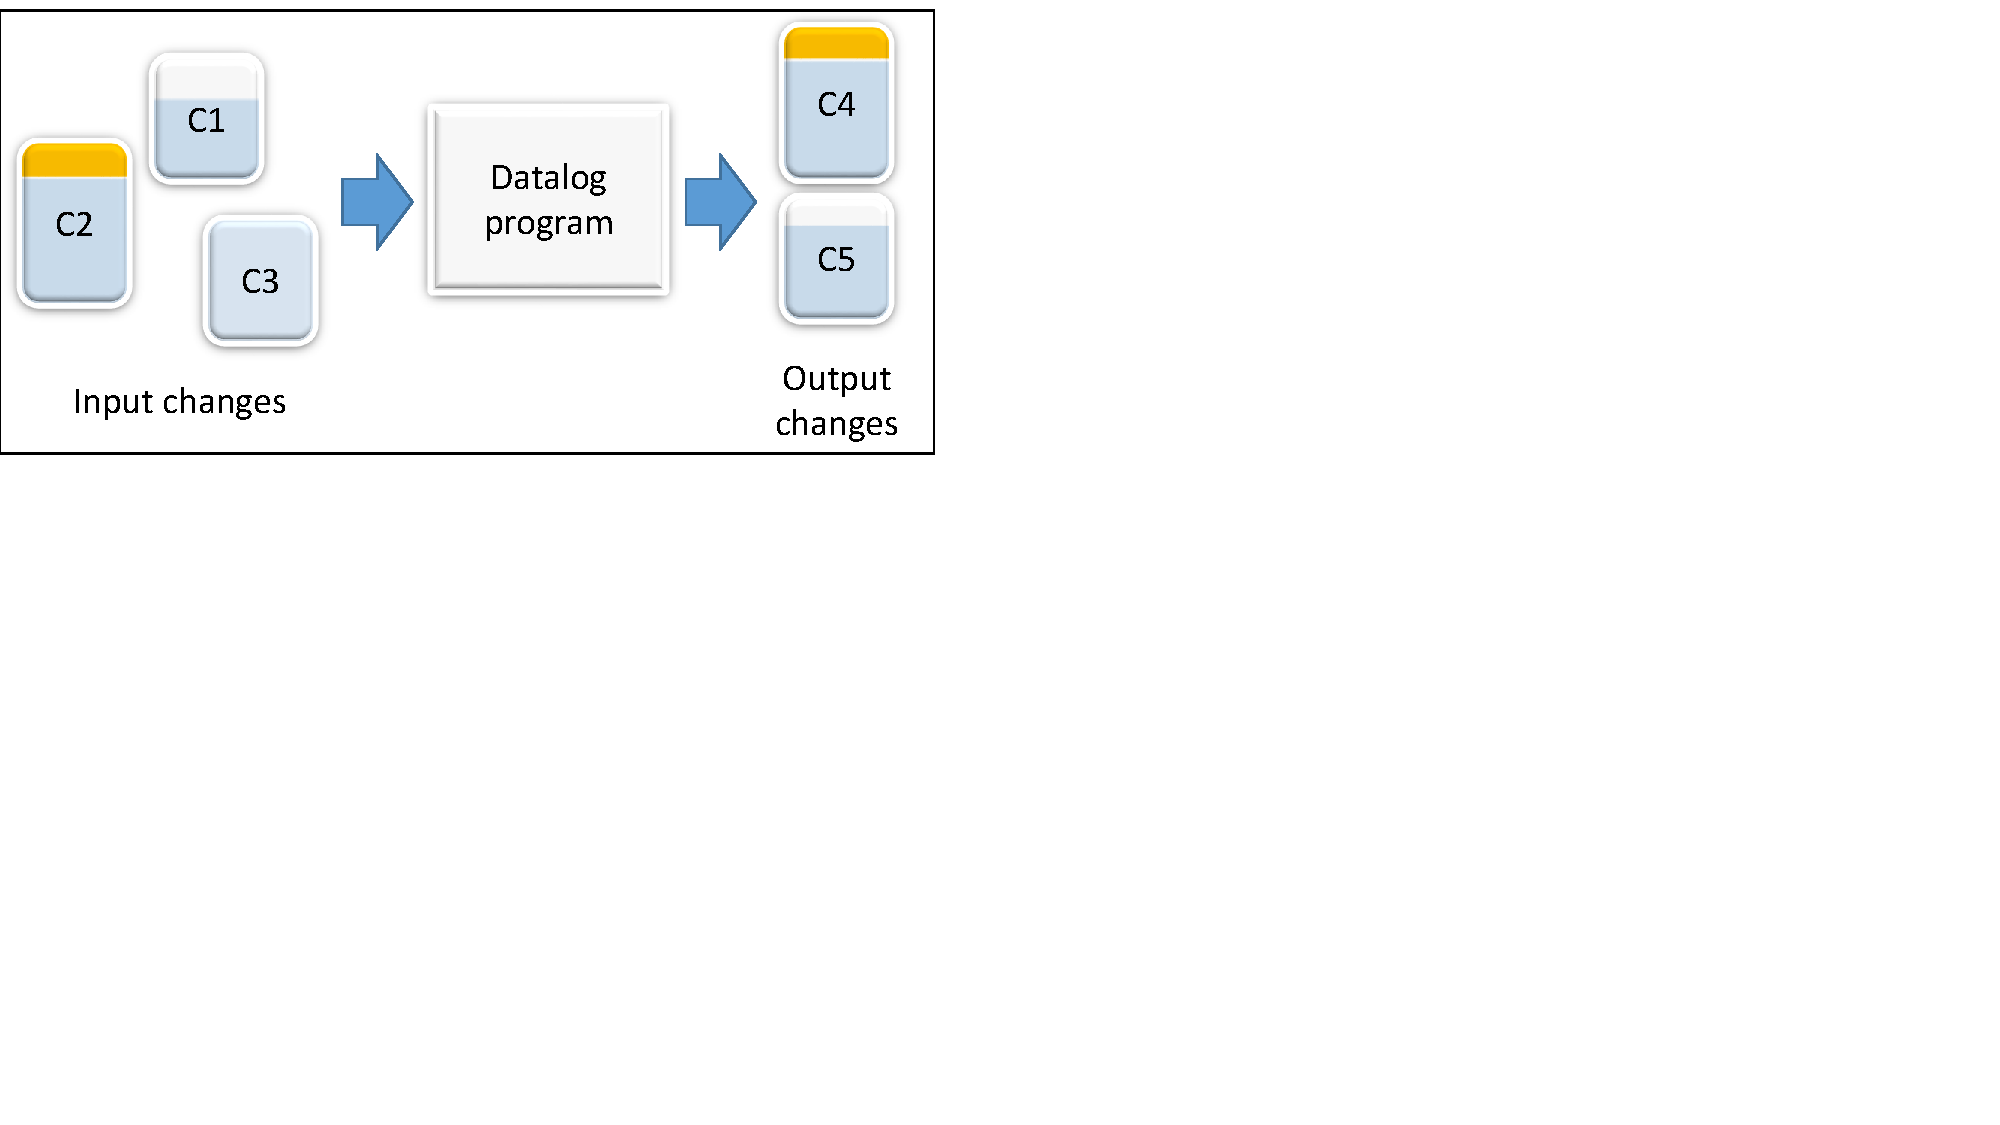
\includegraphics[width=\columnwidth,clip=true,trim=0in 1.6in 6in
      0in]{differential.pdf}
    \caption{Differential computation.\label{fig:differential}}
  \end{minipage} \hfill
  \begin{minipage}{.48\textwidth}
    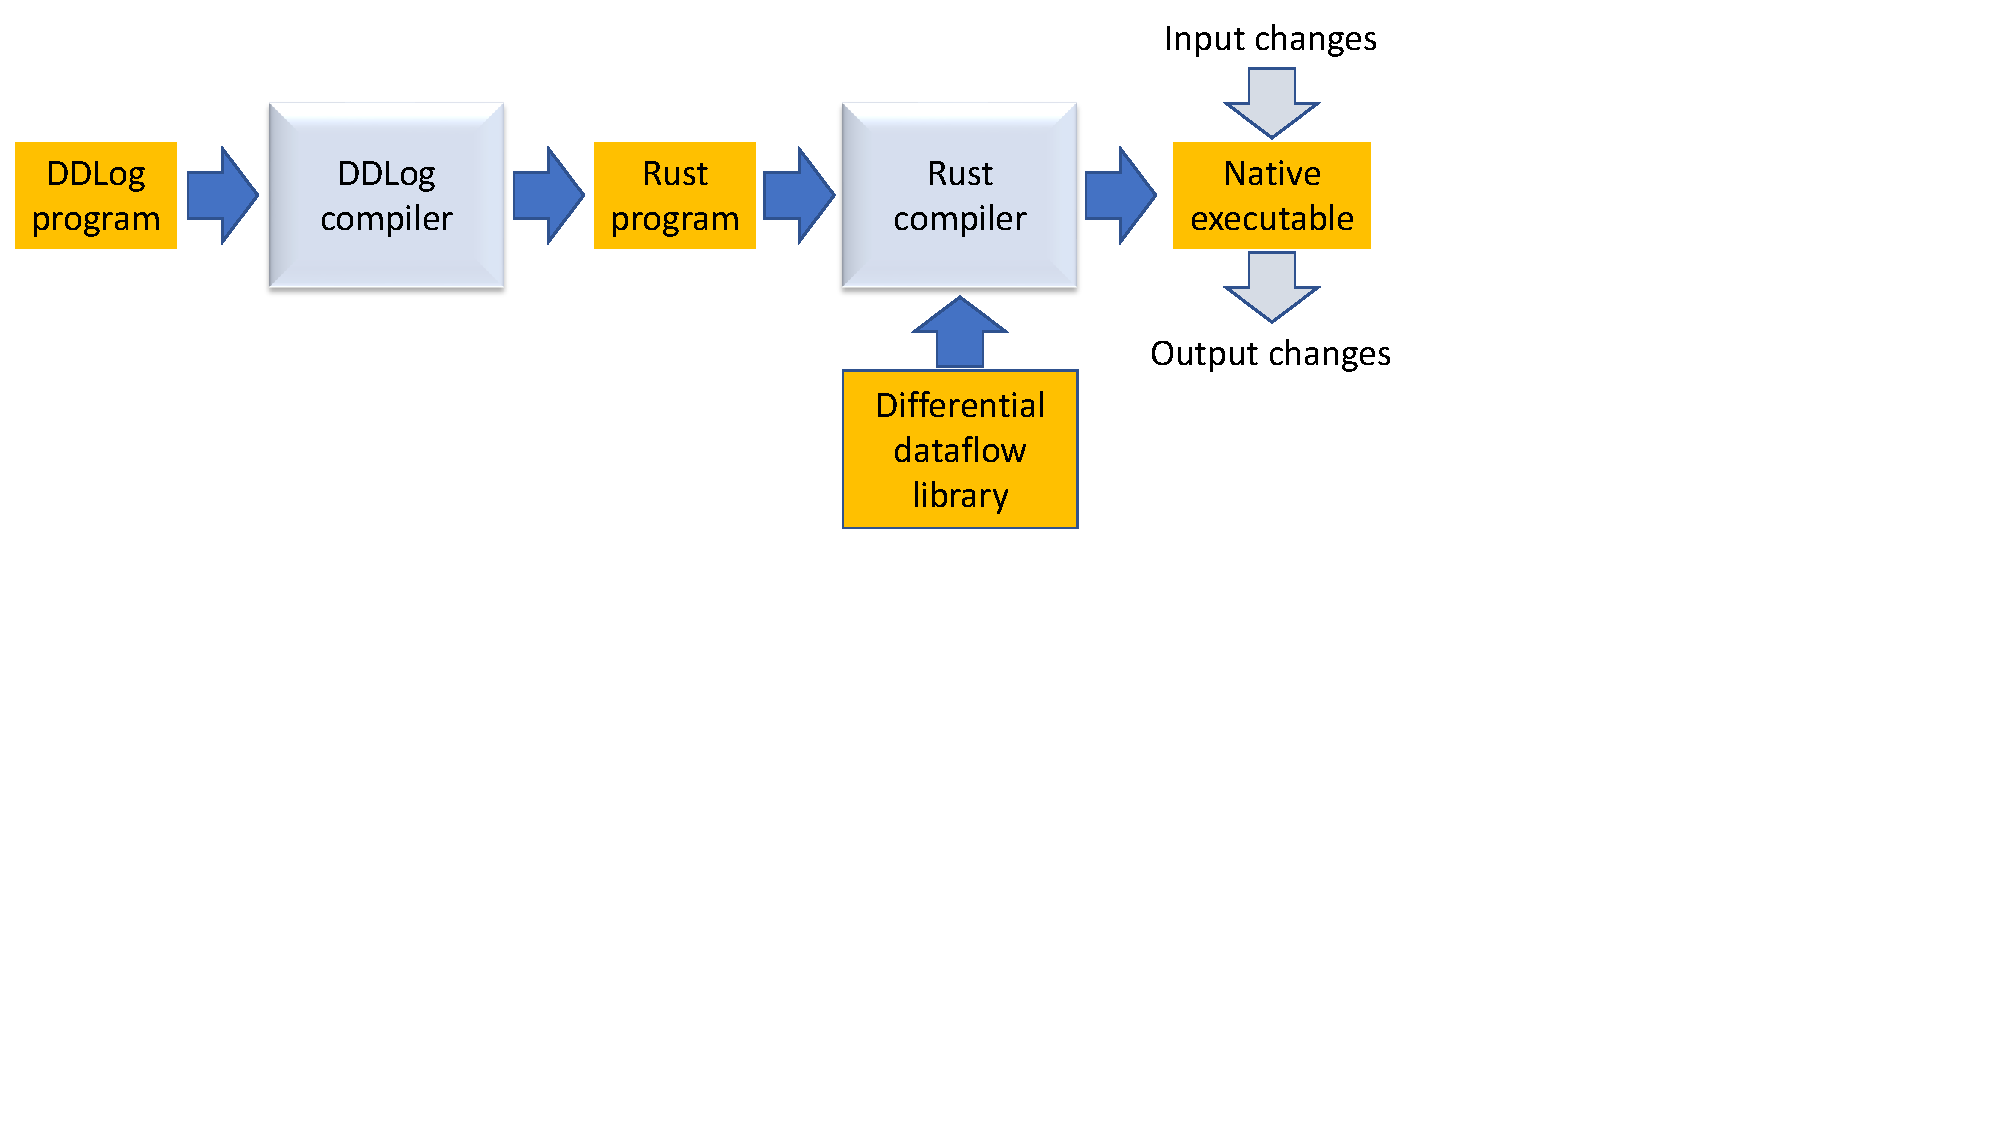
\includegraphics[width=\columnwidth,clip=true,trim=0in 4in 4in
      0in]{compiler-flow.pdf}
    \caption{Compiling DDlog.\label{fig:compiler-flow}}
  \end{minipage}
\end{figure}

In this section we give a brief overview of the language; we refer the
reader to the DDlog language reference~\cite{ddlog-manual} for a
detailed presentation of the syntax, and to the DDlog
tutorial~\cite{ddlog-tutorial}.

\subsection{Syntax}

DDlog is case-sensitive.  Relation, constructor, and type variable
names must start with upper-case ASCII letters; variable, function,
and argument names must start with lower-case ASCII letters or
underscore.  A type variable name must be prefixed with a tick ('). A
type name can start with either an upper-case or a lower-case letter
or underscore.

\subsection{Language restrictions}

We support recursion with stratified negation.

\subsection{Type system}

DDlog is a strongly-typed language.  All programs are type-checked
statically.  The type system is inspired by Haskell, and supports a
rich set of types, but does not support recursive types.

\begin{lstlisting}[language=ddlog]
/* Comments are C++-style */
typedef Color = Red   // an enumerated type
              | Green
              | Blue

// A tagged-union type
typedef IPAddress = IPv4Address{addr: bit<32>} // 32-bit vector
                  | IPv6Address{addr: bit<128>}
                  | None

// The contents of input relations comes from the environment
input relation Mix(c: Color,
                   big: bigint, // arbitrary-precision integer
                   s: string,   // UTF-8 strings
                   b: bool,
                   a: IPAddress)
\end{lstlisting}

\subsubsection{Generic types}

\subsection{Expression language}


\subsection{Pure functions}


\subsection{Control-flow constructs}

\subsection{Extern computations}

\subsection{Module system}
